\documentclass[lettersize,journal]{IEEEtran}
\usepackage[T1]{fontenc}
\usepackage{amsmath,amsfonts,amssymb}
\usepackage{textcomp}
\usepackage{stfloats}
\usepackage{graphicx}
\usepackage{booktabs}
\usepackage{multirow}
\usepackage{array}
\usepackage{url}
\usepackage{cite}
\usepackage[hidelinks]{hyperref}
\graphicspath{{figures/}}
\newcommand{\aucfa}{\mathrm{AUC}^{\mathrm{1st}}}

\begin{document}

\title{When Accurate Prerequisite Graphs Are Not More Useful: Disentangling Structural Quality and Predictive Utility in Knowledge Tracing}

\author{Zineb~Elkaimbillah,
        Sabah~Miqoi,
        Mohamed~Khoual,
        and~Mahmoud~Elhamlaoui%
\thanks{(Corresponding author: Zineb Elkaimbillah.)}%
\thanks{Zineb Elkaimbillah, Mohamed Khoual, and Mahmoud Elhamlaoui are with the IMS Team, ADMIR Laboratory, Rabat IT Center, ENSIAS, Mohammed V University in Rabat, Rabat, Morocco (e-mail: zineb\_elkaimbillah@um5.ac.ma; mohamed\_khoual@um5.ac.ma; mahmoud.elhamlaoui@ensias.um5.ac.ma).}%
\thanks{Sabah Miqoi is with the Team of Embedded Systems, Renewable Energy and Artificial Intelligence, National School of Applied Sciences, Mohammed First University, Oujda, Morocco (e-mail: sabah.miq@gmail.com).}}

\markboth{IEEE Transactions on Learning Technologies}%
{Elkaimbillah \MakeLowercase{\textit{et al.}}: Structural Quality and Predictive Utility of Prerequisite Graphs}

\maketitle

\begin{abstract}
Prerequisite graphs are widely used to improve knowledge tracing (KT) and are increasingly generated by large language models (LLMs) or learned from learner data. These practices often assume, at least implicitly, that a graph that agrees with expert prerequisites is more useful for prediction, and that a graph that helps prediction reveals true prerequisites. We test this assumption by separating the structural quality of a prerequisite graph from its predictive utility, using Junyi Academy, a second real dataset (DBE-KT22) and simulated learners with a known prerequisite structure. Graph effects appear on first attempts in sparse-data regimes. There, in controlled experiments on Junyi that vary coverage, edge correctness and topical proximity at matched in-degrees, coverage explains most of a graph's effect on first-attempt AUC (partial $\eta^2$ 0.70--0.77) and its effect is two to four times that of correctness, although both effects depend on the KT architecture and the evaluation regime; wrong same-topic edges keep about 80\% of the expert graph's benefit. The direction of the effect depends on the architecture: in the regimes studied, the same graphs help a prerequisite-aware model and degrade our implementation of Graph-based Knowledge Tracing. Graphs from two LLMs are more faithful than chance but show no significant advantage over random same-topic graphs at equal coverage. A graph learned end-to-end by a KT model agrees weakly with expert prerequisites (ROC AUC 0.54, at most 0.57 across eleven learning settings) while matching the expert graph's predictive benefit. Under the simulated conditions, edge correctness and direction yielded detectable benefits mainly when prerequisites strongly influenced success, and order- and co-occurrence-based recovery confounded curriculum order with prerequisites. We propose guidelines for evaluating structural quality and predictive utility separately.
\end{abstract}

\begin{IEEEkeywords}
Knowledge tracing, prerequisite graphs, large language models, learner modeling, evaluation methodology, interpretability, adaptive learning.
\end{IEEEkeywords}

\section{Introduction}
\IEEEPARstart{K}{nowledge} tracing (KT) models estimate what a learner knows from the sequence of their answers and predict whether they will answer the next item correctly. These predictions drive adaptive learning systems: which exercise to propose next, when to review, when a learner is ready to move on. A recurring idea in KT research is that models predict better when they know how knowledge is structured, and in particular which items are prerequisites of others: if a learner has failed the prerequisite of an exercise they have never attempted, the model should expect them to struggle. Many graph-based KT models therefore take a prerequisite or concept graph as input, or learn one jointly with prediction~\cite{chen2018prerequisite,nakagawa2019graph,tong2020structure,zhou2024predictive}.

Expert prerequisite graphs are expensive to build, and two cheaper sources have become common. LLMs can be asked whether one concept is a prerequisite of another, producing graphs at scale~\cite{aytekin2025discovering,le2025llms}. Alternatively, a KT model can learn edge weights from learner data, and the learned structure is often presented as interpretable pedagogical knowledge. Both practices often rest, at least implicitly, on an assumption that is rarely tested directly: that a graph's \emph{structural quality}, its agreement with expert prerequisites, and its \emph{predictive utility} for KT go together. Under this assumption, a more accurate LLM graph should be more useful, and a learned graph that improves prediction should reveal true prerequisites. For learning technologies the distinction matters beyond prediction: prerequisite graphs are also used to sequence content, to justify recommendations to learners and teachers, and to plan remediation, uses for which a graph that is merely predictive may be misleading.

This paper tests that assumption (Fig.~\ref{fig:overview}). We define structural quality and predictive utility formally and measure how they relate under controlled conditions on Junyi Academy, the main public dataset that combines learner interactions with expert-annotated directed prerequisites, on a university course dataset (DBE-KT22), and on simulated learners whose prerequisite structure is known. We ask four research questions: how faithful LLM-generated graphs are (RQ1); which properties of a graph, among coverage, edge correctness and topical proximity, make it useful (RQ2); whether the answer depends on the KT architecture (RQ3); and whether graphs learned from data recover prerequisites, and whether their utility reflects their fidelity (RQ4).

\begin{figure*}[t]
\centering
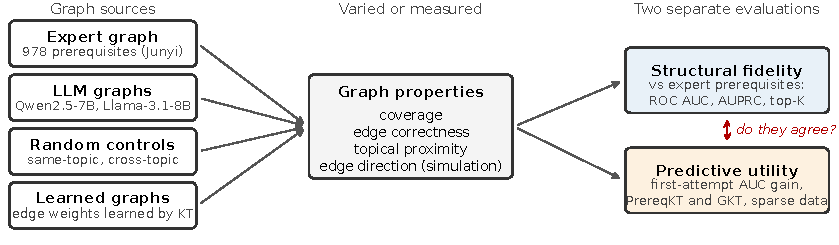
\includegraphics[width=0.92\textwidth]{fig1_overview.pdf}
\caption{Overview of the study. Graphs from four sources are characterized by controlled properties and evaluated on two separate axes: structural fidelity to expert prerequisites and predictive utility for KT.}
\label{fig:overview}
\end{figure*}

We find that an expert graph brings no measurable gain with full data and all interactions, but helps on first attempts in sparse-data regimes. There, structural quality and predictive utility largely dissociate: coverage explains most of a graph's effect, the same graphs help one architecture and degrade another in our implementation, LLM graphs show no advantage over random same-topic graphs once coverage is equalized, and a learned graph matches the expert graph's benefit while barely recovering expert prerequisites. Our contributions are:
\begin{enumerate}
\item a formal separation of the structural quality and predictive utility of prerequisite graphs, with first-attempt-weighted coverage, correctness, proximity, utility and fidelity measures;
\item a controlled factorial study that quantifies the contributions of coverage, correctness and proximity to KT utility, replicated with a second architecture and a second dataset;
\item an audit of LLM-generated prerequisite graphs from two model families, for both fidelity and utility;
\item evidence, on real and simulated data, that learned graphs can be predictively useful without recovering prerequisites, with an analysis of why log-based recovery methods fail;
\item evaluation guidelines for studies that use or produce prerequisite graphs for KT.
\end{enumerate}

\section{Related Work}
\subsection{Knowledge Tracing and Graph-Based Models}
Classical KT approaches include Bayesian Knowledge Tracing~\cite{corbett1994knowledge} and logistic models such as Performance Factors Analysis~\cite{pavlik2009performance}. Deep Knowledge Tracing~\cite{piech2015deep} introduced recurrent networks, followed by memory-augmented~\cite{zhang2017dynamic} and attention-based models~\cite{pandey2019self,ghosh2020context}. A substantial line of work injects relations between items or concepts: prerequisite-driven KT constrains predictions with prerequisite relations~\cite{chen2018prerequisite}; Graph-based Knowledge Tracing (GKT) propagates learner states over a concept graph~\cite{nakagawa2019graph}; later models use graph neural networks over question--concept, concept--concept or hierarchical exercise graphs~\cite{yang2020gikt,tong2020structure,tong2022introducing}. These models are typically evaluated by overall AUC against graph-free baselines, and the contribution of the graph is rarely separated from that of its density or coverage.

\subsection{Learning Prerequisite Structure}
Prerequisite relations have been inferred from text and course material, such as Wikipedia links~\cite{liang2015measuring}, MOOC transcripts~\cite{pan2017prerequisite}, lecture collections~\cite{li2019lecturebank} and online resources~\cite{roy2019inferring}. From learner data, they have been inferred from performance statistics~\cite{vuong2011method,scheines2014discovering}, interpretable learner models~\cite{allegre2023discovering}, causal discovery~\cite{yu2024causal} and KT models themselves~\cite{tong2020structure,zhou2024predictive}. The Junyi Academy data~\cite{chang2015modeling} is the main public resource with expert prerequisite annotations. PSI-KT~\cite{zhou2024predictive} learns an interpretable prerequisite structure jointly with prediction and evaluates its alignment with Junyi's annotations. The replication materials of Truong~\cite{truong2026replication}, released with a study not yet published in a peer-reviewed venue, report that prerequisite relations are poorly recovered from correctness logs on Junyi and that supplied graphs bring small gains comparable to topic-matched and reversed controls. We share this concern and differ in four respects: we identify the conditions under which a graph matters (first attempts, sparse data), isolate coverage, correctness and proximity in a factorial design and quantify their relative weight, show that the direction of the effect depends on the architecture, and explain the observed patterns with a simulation whose ground truth is known.

\subsection{LLMs for Educational Knowledge Structures}
LLMs are increasingly used to generate concept maps, prerequisite relations and knowledge graphs for education, usually evaluated against expert annotations on concept pairs or skill lists~\cite{aytekin2025discovering,le2025llms,yang2025examining}. Evidence on whether such graphs improve downstream learner modeling is scarce; we evaluate graphs from two LLM families for both fidelity and KT utility.

\subsection{Evaluation Practice}
Conclusions about KT models depend on evaluation choices, dataset properties and baselines~\cite{khajah2016deep,wilson2016back,pelanek2017bayesian,gervet2020deep,liu2022pykt}. We add two such choices for graph-based KT: evaluating first attempts in sparse regimes, and comparing with coverage-matched random graphs and a difficulty-only reference. More broadly, our distinction between predictive utility and structural validity echoes debates on whether internal structures of predictive models, such as attention weights, constitute explanations~\cite{jain2019attention}: good predictive performance does not by itself validate the structure a model relies on. Table~\ref{tab:position} positions this study.

\begin{table*}[t]
\centering
\caption{Positioning of This Study}
\label{tab:position}
\footnotesize
\setlength{\tabcolsep}{3pt}
\begin{tabular}{@{}p{2.9cm}p{2.7cm}p{3.2cm}p{2.6cm}p{2.9cm}p{1.6cm}@{}}
\toprule
Work & Graph sources & Evaluation of utility & Evaluation of structure & Controlled factors & Simulation \\
\midrule
Graph-based KT models, e.g.,~\cite{nakagawa2019graph,yang2020gikt,tong2020structure} & Expert or data-derived & Overall AUC & Rarely & No & No \\
PSI-KT~\cite{zhou2024predictive} & Learned & Prediction & Alignment with Junyi annotations & No & No \\
Truong~\cite{truong2026replication} & Expert, annotator, log-derived & Overall AUC, controls & Recovery from logs & Random, topic-matched, reversed controls & Yes \\
This study & Expert, two LLMs, random controls, learned & First-attempt AUC in sparse regimes, two architectures, difficulty reference & ROC AUC, AUPRC, top-$K$ precision & Coverage $\times$ correctness $\times$ proximity at matched in-degrees & Yes, three scenarios \\
\bottomrule
\end{tabular}
\end{table*}

\section{Problem Formulation}
\subsection{First-Attempt Evaluation}
Let $Q=\{q_1,\dots,q_n\}$ be the items of a platform. Each learner produces a chronological sequence of interactions $(q_t, r_t)$, $r_t\in\{0,1\}$. A KT model $f$ estimates $\hat p_{t+1}=f(q_{t+1}\mid (q_1,r_1),\dots,(q_t,r_t);G)$, where $G$ is an optional prerequisite graph supplied to, or learned by, the model. An interaction is a \emph{first attempt} if the learner has not attempted $q_t$ before. On a first attempt the history contains no information about the target item, so any information about it must come from other items. First attempts are therefore the most direct test of what a graph contributes; graphs may also help on later attempts, but there their contribution is mixed with that of the item's own history. We report the ROC AUC over all first attempts in the test set ($\aucfa$) and vary the amount of training data by sampling a fraction $\rho$ of the training learners.

\subsection{Graphs and Their Properties}
A prerequisite graph is a directed graph $G=(Q,E)$ in which $(a,b)\in E$ states that $a$ is a prerequisite of $b$. $E^*$ is the expert-annotated graph (``expert prerequisites'' for short; on DBE-KT22 we speak of reference relations, and in the simulation of ground-truth prerequisites) and $\mathrm{anc}^*(b)$ the set of direct and indirect expert prerequisites of $b$. Each item has a topic $\tau(b)$. The candidate set $C$ contains all ordered pairs of distinct items sharing a topic; a \emph{scored graph} assigns a score $s(a,b)$ to every pair in $C$ (an LLM probability or a learned weight). We characterize a graph by three properties that can be varied independently. \emph{Coverage} is weighted by the first attempts it can affect: with $w_b$ the number of test first attempts on $b$,
\begin{equation}
\mathrm{Cov}(G)=\frac{\sum_b w_b\,\mathbb{1}[\deg^-_G(b)>0]}{\sum_b w_b}.
\end{equation}
\emph{Edge correctness} is $|E\cap E^*|/|E|$ (extended form: $a\in\mathrm{anc}^*(b)$), and \emph{topical proximity} is the share of edges whose endpoints share a topic.

\subsection{Utility and Fidelity}
The \emph{predictive utility} of $G$ for model $f$ and fraction $\rho$ is
\begin{equation}
U_{f,\rho}(G)=\aucfa_{f,\rho}(G)-\aucfa_{f,\rho}(\varnothing),
\end{equation}
and the \emph{benefit retained} is $U(G)/U(E^*)$. Utility is a property of a graph \emph{together with} a model. The \emph{structural fidelity} of a scored graph is its ability to rank expert prerequisites above other candidates, measured by ROC AUC, the area under the precision--recall curve (AUPRC) and precision among the $K=|E^*\cap C|$ highest-scoring pairs. Chance corresponds to 0.5 (ROC AUC) and to the positive rate (AUPRC). Low fidelity indicates weak agreement with an expert reference that may itself be incomplete, not proof that the relations are pedagogically wrong. \emph{Recoverability} is the fidelity of a graph learned from learner data.

\subsection{Research Questions and Hypotheses}
The common assumption behind graph-based KT is that fidelity and utility go together. We test it through four research questions:
\begin{itemize}
\item \textbf{RQ1:} How faithful to expert prerequisites are LLM-generated graphs, and how are their edges distributed across items?
\item \textbf{RQ2:} When coverage, edge correctness and topical proximity are varied independently at matched in-degrees, how much does each contribute to predictive utility?
\item \textbf{RQ3:} Do the answers to RQ2 hold across KT architectures that use the graph in different ways?
\item \textbf{RQ4:} Can prerequisites be recovered from learner data, and does a learned graph's utility reflect its fidelity?
\end{itemize}
A simulation with known prerequisites addresses an explanatory question across RQ2 and RQ4: under which conditions does correctness matter, and when can prerequisites be recovered?

The study was iterative: preliminary experiments, which led us to evaluate first attempts in sparse regimes, were exploratory. For each controlled experiment that followed, the primary hypotheses (Table~\ref{tab:hyp}) were fixed before running it, without formal registration, and tested with Holm correction over that experiment's primary tests. Only the tests of H1--H8 are confirmatory. All other analyses are exploratory: the choice of first attempts and sparse regimes, the LLM-versus-random comparisons, pairwise and averaged comparisons, effect-magnitude ratios, the DBE-KT22 replication, the simulation, the shape of learned graphs and the sensitivity analysis. Where results contradicted a directional hypothesis, we also report two-sided tests, identified as such.

\begin{table}[t]
\centering
\caption{Pre-Specified Primary Hypotheses}
\label{tab:hyp}
\footnotesize
\setlength{\tabcolsep}{3pt}
\begin{tabular}{@{}p{1.5cm}p{4.45cm}p{1.45cm}@{}}
\toprule
Experiment & Hypothesis & Test \\
\midrule
Factorial (RQ2) & H1, coverage: expert edges at 100\% $>$ at 25\% coverage & One-sided paired $t$ \\
 & H2, correctness does not matter: expert $\approx$ wrong same-topic edges at 100\% & TOST, margin 20\% of expert gain \\
 & H3, proximity: wrong same-topic $>$ wrong cross-topic edges at 100\% & One-sided paired $t$ \\
Second model (RQ3) & H1--H3, plus H4: wrong cross-topic edges $>$ no graph & One-sided paired $t$ \\
Learned (RQ4) & H5: learned weights rank expert prerequisites above chance & One-sided $t$ vs.\ 0.5 \\
 & H6: learned weights outperform practice order & One-sided paired $t$ \\
 & H7: training on learner data improves an LLM prior & One-sided paired $t$ \\
 & H8: recovery above chance on pairs without imposed order & One-sided $t$ vs.\ 0.5 \\
\bottomrule
\end{tabular}
\end{table}

\section{Data}
Table~\ref{tab:data} summarizes the datasets. \textbf{Junyi Academy}~\cite{chang2015modeling} is a Taiwanese mathematics platform whose 2015 release includes, for each exercise, the prerequisite exercises defined by content experts; to our knowledge it is the only public KT dataset that combines interactions with expert-annotated directed prerequisites~\cite{zhou2024predictive}. We sample 20{,}000 learners with at least ten interactions, cut sequences at 200 interactions and split learners 70/10/20\%. The candidate set $C$ contains 22{,}760 same-topic pairs and includes 83.8\% of the 978 expert edges.

\textbf{DBE-KT22}~\cite{abdelrahman2022dbe} records answers of university students to 212 questions of a relational databases course, linked to 98 knowledge components (KCs). Its 202 KC relations all appear in both directions, so they encode relatedness rather than prerequisites. We link question $a$ to $b$ if a KC of $a$ is related to a KC of $b$ and they share no KC (1{,}368 links), use quizzes as topics, and keep 1{,}140 students. DBE-KT22 therefore tests graphs of related knowledge, not directed prerequisites.

\textbf{Simulated learners.} A synthetic curriculum of 120 items in six topics has a directed acyclic prerequisite graph of 201 edges (one to three prerequisites per item, 85\% within topic). The generator, an item-response model with learning, differs from the evaluated KT models:
\begin{equation}
P(r=1)=\sigma\!\big(0.8+\theta+\theta_{\tau(k)}-d_k+2m_k-\lambda(1-\bar m_{\mathrm{pre}(k)})\big),
\end{equation}
where $\theta,\theta_\tau$ are general and topic abilities, $d_k$ the difficulty, $m_k\in[0,1]$ the mastery of $k$ and $\bar m_{\mathrm{pre}(k)}$ the mean mastery of its prerequisites. After each attempt mastery increases by $0.5g$ (20\% more after a success), with $g=0.3+0.7\bar m_{\mathrm{pre}(k)}$ when $\lambda>0$ and $g=1$ when $\lambda=0$. Three scenarios with 3{,}000 learners each vary prerequisite strength and practice order: S1, strong prerequisites ($\lambda=2$, free order); S2, weak prerequisites ($\lambda=0.7$, free order); S3, no prerequisite effect on success or learning ($\lambda=0$) with an imposed curriculum order. S3 changes both factors at once (Section~\ref{sec:limits}).

\begin{table}[t]
\centering
\caption{Datasets}
\label{tab:data}
\footnotesize
\setlength{\tabcolsep}{3pt}
\begin{tabular}{@{}p{1.55cm}p{2.05cm}p{2.05cm}p{1.75cm}@{}}
\toprule
 & Junyi Academy & DBE-KT22 & Simulation \\
\midrule
Domain & School mathematics & University databases & Synthetic \\
Learners & 20{,}000 (sample) & 1{,}140 & 3{,}000 per scenario \\
Items & $\approx$800 exercises & 212 questions & 120 items \\
Reference graph & 978 directed expert prerequisites & 202 symmetric KC relations & 201 directed prerequisites \\
Topics & Platform topics & 10 quizzes & 6 topics \\
Fractions $\rho$ & 1\%, 5\% (100\%) & 5\%, 20\% (100\%) & 5\%, 20\% (100\%) \\
\bottomrule
\end{tabular}
\end{table}

\section{Methods}
\subsection{KT Models Used as Instruments}
The two models below are experimental probes, not proposed architectures; they use a graph in contrasting ways. PrereqKT exposes prerequisite information through explicit features, which allows us to isolate how coverage and correctness affect prediction; GKT routes all information between items through the graph. \textbf{PrereqKT} is a recurrent model whose item embeddings (dimension 64) are refined over two layers by separate channels from prerequisites and successors (row-normalized adjacency), read by a long short-term memory network~\cite{hochreiter1997long} (hidden size 128). Its prediction for item $b$ also receives six indicators from the learner's history: over $b$'s prerequisites, the mean success rate on those attempted, the share attempted and whether $b$ has prerequisites, and the same over successors. With an empty graph it reduces to a recurrent model with item embeddings. Training uses Adam~\cite{kingma2015adam} (learning rate $10^{-3}$), batches of 64, dropout 0.2, at most 60 epochs and early stopping on validation AUC (patience 5). \textbf{GKT}~\cite{nakagawa2019graph} is re-implemented in its fixed-graph variant (dimension 32): an answer updates the hidden states of the answered item and of its neighbours through separate message functions towards prerequisites and successors, an erase--add gate and a gated recurrent unit~\cite{cho2014learning}. Without a graph, information does not flow between items. Our one adaptation is a learned initial state per item, without which all first attempts would receive the same prediction in the no-graph condition.

\subsection{Graph Conditions}
\textbf{Factorial graphs (RQ2, RQ3).} For a \emph{coverage level} $c\in\{25,50,100\%\}$ we select a nested random subset of $c$ of the items that have expert prerequisites; each selected item receives as many incoming edges as it has expert prerequisites, so in-degrees are matched across sources. The resulting first-attempt-weighted coverage is 21.9, 43.5 and 87.2\% on Junyi for all sources. Incoming edges come from the item's \emph{expert} prerequisites, from \emph{wrong same-topic} items (neither direct nor indirect prerequisites), or from \emph{wrong cross-topic} items. At full coverage the sources contain 978, 972 and 978 edges: in a few small topics too few eligible items exist, so the same-topic source lacks about six edges. On DBE-KT22, quizzes are too small for a matched same-quiz control, so the matched comparison is reference relations against wrong cross-quiz links; the simulation adds a \emph{reversed} source (successors instead of prerequisites).

\textbf{LLM graphs (RQ1).} Each pair $(a,b)\in C$ is presented to Qwen2.5-7B-Instruct~\cite{qwen2024qwen25} and Llama-3.1-8B-Instruct~\cite{grattafiori2024llama}, both quantized to 4 bits~\cite{dettmers2023qlora}, with the names and topics of the two exercises and the question whether a student must master $a$ before attempting $b$. The score is the probability of ``Yes'' from the next-token logits, normalized over ``Yes'' and ``No''. Graphs keep either the highest-scoring pairs globally, or each item's $k\in\{1,2,3,5\}$ best-scored prerequisites, which makes coverage complete. \textbf{Random controls} draw the same number of sources per item (or edges in total) uniformly among same-topic candidates.

\textbf{Learned graphs (RQ4).} In a variant of PrereqKT every pair in $C$ receives a weight $w_{ab}=\sigma(\theta_{ab})$ that replaces the binary adjacency, with the loss
\begin{equation}
\mathcal L=\mathcal L_{\mathrm{BCE}}+\lambda_1\overline{w}+\lambda_{\mathrm{acyc}}\big(\operatorname{tr}e^{W\circ W}-n\big),
\end{equation}
where the last term is the NOTEARS acyclicity penalty~\cite{zheng2018dags}, $\lambda_1=\lambda_{\mathrm{acyc}}=0.01$ and the edge learning rate is $10^{-2}$. Weights start at 0.1 (no prior) or at the Qwen score (LLM prior). A sensitivity analysis varies $\lambda_1,\lambda_{\mathrm{acyc}}\in\{0,0.01,0.1\}$, the initial weights and the candidate set; the setting to report was fixed in advance as the one with the best KT validation AUC. We compare learned weights with statistics computed on the training logs: \emph{practice order}, the share of learners who attempt $a$ before $b$, and, in the simulation, \emph{co-occurrence lift} (difference in first-attempt success on $b$ between learners who succeeded and failed on $a$) and \emph{practice-before} (difference in first-attempt success on $b$ between learners who attempted $a$ before and after $b$). On Junyi, pairs attempted by at least 20 learners have an \emph{imposed order} when at least 95\% follow the same order, and a \emph{variable order} otherwise.

\textbf{Difficulty-only reference.} Each first attempt is predicted by the item's smoothed success rate among the sampled training learners, with no history and no graph.

\subsection{Statistical Analysis}
The seed fixes both the sampled training learners and the initialization, so comparisons are paired by seed. All seeds share the same test learners: seeds are not independent test samples, and intervals reflect training variability rather than the uncertainty of sampling new students. We use 10 seeds for the factorial and architecture experiments and 5 for the others. We report means, 95\% bootstrap intervals over seeds~\cite{efron1993introduction} and the number of seeds favoring one condition. Primary hypotheses use paired $t$-tests with Holm correction~\cite{holm1979simple}; equivalence uses two one-sided tests (TOST)~\cite{schuirmann1987comparison,lakens2017equivalence} with a margin of 20\% of the expert gain. In the factorial design, a two-way ANOVA of the gain over no graph (coverage, source, interaction, seed as block) gives partial $\eta^2$, a share of explained variance reported separately from AUC gains. When comparing effect magnitudes across architectures whose graph effect has opposite signs, effects are oriented in the direction of the expert graph's effect. Experiments used PyTorch~\cite{paszke2019pytorch} on NVIDIA T4 GPUs; the code, notebooks and result files are available from the corresponding author upon reasonable request.

\section{Results}
\subsection{Where a Prerequisite Graph Can Matter}
With all training learners and all interactions, the expert graph brings no measurable gain on Junyi (test AUC 0.8028 with the expert graph, 0.8026 without a graph, 0.8027 with a random graph), consistent with the near-null gains reported for supplied graphs in full-data settings~\cite{truong2026replication}. On first attempts in sparse regimes, the expert graph raises $\aucfa$ of PrereqKT by 0.010 to 0.026, and the gain grows as training data shrink (Table~\ref{tab:sparse}); a global random graph of the same size brings a third to a half of these gains.

\begin{table}[t]
\centering
\caption{First-Attempt AUC on Junyi (PrereqKT, 5 Seeds)}
\label{tab:sparse}
\footnotesize
\setlength{\tabcolsep}{3.5pt}
\begin{tabular}{@{}lcccc@{}}
\toprule
Learners & No graph & Random & Expert & Expert $-$ none \\
\midrule
10\% & 0.7796 & 0.7850 & 0.7892 & +0.010 \\
5\% & 0.7655 & 0.7692 & 0.7768 & +0.011 \\
1\% & 0.7050 & 0.7160 & 0.7314 & +0.026 \\
\bottomrule
\end{tabular}
\end{table}

 Against the difficulty-only reference (10 seeds), PrereqKT with the expert graph wins at $\rho=5\%$ (0.7774 vs.\ 0.7655, 10 of 10 seeds) but only matches it at 1\% (0.7283 vs.\ 0.7283), where GKT without a graph is the strongest predictor (0.7434): in the sparsest regime the graph mainly compensates for poorly estimated item difficulty. All comparisons below use $\aucfa$ at $\rho=5\%$ and 1\% on Junyi.

\subsection{Fidelity and Utility of LLM Graphs (RQ1)}
Both LLMs rank expert prerequisites above chance, Qwen more than Llama (Table~\ref{tab:llm}). Among the 978 highest-scoring pairs (the size of the expert graph), 11.2\% (Qwen) and 8.8\% (Llama) are expert prerequisites, against 3.6\% at random; counting indirect prerequisites, precision reaches 44.0\% and 32.2\% (17.6\% at random). The two models disagree on which pairs are prerequisites (Spearman 0.59 between scores; Jaccard overlap of the top-978 sets 0.19), and averaging their scores does not improve fidelity (ROC AUC 0.693). Fidelity does not translate into utility. The most confident Qwen graph (top 978 pairs) retains $-4\%$ ($\rho=5\%$) and 14\% (1\%) of the expert graph's benefit, because its edges concentrate on a few foundational exercises and leave most items uncovered (first-attempt coverage 24\%). Larger graphs perform as well as the expert graph (top 7{,}824 pairs: 117\% and 89\%), but so do random same-topic graphs of the same size (82\% and 89\%; 0 of 8 comparisons significant after Holm correction). When each item keeps its $k$ best-scored prerequisites, so that coverage is complete, neither LLM shows an advantage over random same-topic prerequisites (Fig.~\ref{fig:llm}): 0 of 8 Qwen-versus-random and 0 of 16 Llama comparisons are significant, with differences between $-0.008$ and $+0.003$ AUC, although per-item Qwen graphs are three times more precise than random ones (17.2\% vs.\ 4.9\% for $k=1$).

\begin{table}[t]
\centering
\caption{Structural Fidelity of LLM Scores on the 22{,}760 Candidate Pairs of Junyi}
\label{tab:llm}
\footnotesize
\resizebox{\columnwidth}{!}{%
\begin{tabular}{@{}lccc@{}}
\toprule
Measure & Qwen2.5-7B & Llama-3.1-8B & Chance \\
\midrule
ROC AUC, direct prerequisites & 0.695 & 0.644 & 0.500 \\
ROC AUC, direct or indirect & 0.670 & 0.627 & 0.500 \\
Precision, top 978 & 11.2\% & 8.8\% & 3.6\% \\
Extended precision, top 978 & 44.0\% & 32.2\% & 17.6\% \\
Reversed edges, top 978 & 7.7\% & 10.2\% & 17.6\% \\
Pairs answered ``Yes'' ($s\ge0.5$) & 31.5\% & 41.6\% & -- \\
Pairs with $s\ge0.999$ & 5.5\% & 0.0\% & -- \\
First-attempt coverage, top 978 & 24.2\% & 21.0\% & -- \\
Edges from the 10 most frequent sources & 22.6\% & 19.1\% & -- \\
\bottomrule
\end{tabular}}
\end{table}

\begin{figure}[t]
\centering
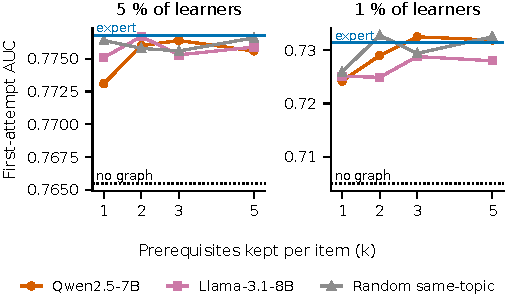
\includegraphics[width=\columnwidth]{fig2_llm_topk.pdf}
\caption{First-attempt AUC of per-item graphs that keep each item's $k$ best-scored prerequisites, for two LLMs and random same-topic prerequisites (PrereqKT, Junyi, 5 seeds). Lines mark the expert graph and no graph.}
\label{fig:llm}
\end{figure}

\subsection{Coverage, Correctness and Proximity (RQ2)}
Coverage explains most of a graph's effect (Fig.~\ref{fig:factorial}, Table~\ref{tab:factorial}). The ANOVA attributes a partial $\eta^2$ of 0.77 ($\rho=5\%$) and 0.70 (1\%) to coverage, 0.37 and 0.34 to the edge source, with no significant interaction ($p=0.77$ and $0.056$). Raising expert coverage from 25\% to 100\% increases $\aucfa$ by 0.010 and 0.018 in 10 of 10 seeds (H1, Holm $p<0.001$). Correctness has a real but secondary effect: equivalence of expert and wrong same-topic edges (H2) is not established, since the differences (0.0026, 0.0047) are of the size of the margins (0.0027, 0.0054) and expert edges win in 8 of 10 seeds; averaged over coverage levels (exploratory), expert edges win at $\rho=5\%$ (+0.0020, Holm $p=0.009$) but not at 1\% (+0.0017, $p=0.31$). Proximity shows a trend at full coverage (H3: +0.0021, +0.0055, Holm $p=0.11$) and is significant averaged over coverage levels (Holm $p=0.009$, 0.011). Oriented in the direction of the graph's effect, the coverage effect is 3.9 times the correctness effect in both regimes (Table~\ref{tab:magnitude}). These sizes explain the LLM results: the precision advantage of LLMs over random same-topic edges is worth at most a few points of retained benefit, below seed-to-seed variability.

\begin{figure}[t]
\centering
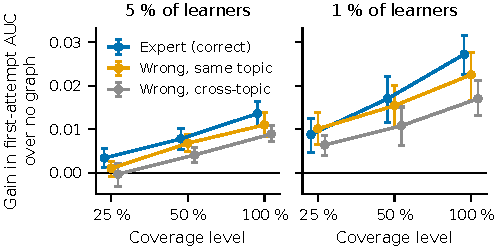
\includegraphics[width=\columnwidth]{fig3_factorial.pdf}
\caption{Factorial design on Junyi (PrereqKT, 10 seeds): gain in first-attempt AUC over no graph by coverage level (share of target items) and edge source, at matched in-degrees; 95\% bootstrap intervals.}
\label{fig:factorial}
\end{figure}

\begin{table}[t]
\centering
\caption{Gain in First-Attempt AUC Over No Graph at Full Coverage (PrereqKT, Junyi, 10 Seeds, 95\% CI) and Share of the Expert Gain}
\label{tab:factorial}
\footnotesize
\setlength{\tabcolsep}{3pt}
\resizebox{\columnwidth}{!}{%
\begin{tabular}{@{}lcccc@{}}
\toprule
Edge source & $\rho=5\%$ & Share & $\rho=1\%$ & Share \\
\midrule
Expert & +0.0136 [0.0107, 0.0163] & 100\% & +0.0272 [0.0225, 0.0314] & 100\% \\
Wrong, same topic & +0.0110 [0.0083, 0.0138] & 81\% & +0.0225 [0.0165, 0.0277] & 83\% \\
Wrong, cross-topic & +0.0089 [0.0071, 0.0109] & 65\% & +0.0170 [0.0131, 0.0212] & 63\% \\
\bottomrule
\end{tabular}}
\end{table}

\subsection{Dependence on the Architecture (RQ3)}
With our implementation of GKT, in the regimes studied, every graph lowers $\aucfa$, and the more a graph covers items and the more accurate it is, the larger the loss (Fig.~\ref{fig:arch}). At $\rho=1\%$ the full-coverage expert graph costs 0.040 (0.7038 vs.\ 0.7434 without a graph), wrong same-topic edges 0.029 and wrong cross-topic edges 0.008; at 5\% the losses are 0.010, 0.008 and 0.004. All directional hypotheses stated as gains are rejected, and the two-sided effects are significant losses (Holm $p<0.05$ for all eight tests). The ordering of factors is nevertheless preserved: the coverage effect is 2.6 and 2.2 times the correctness effect (Table~\ref{tab:magnitude}). The loss is not due to under-training: with up to 200 epochs, training stopped after 64 and 58 epochs with identical results. At $\rho=1\%$, the three runs of one seed (seed 3) failed to train, which we define as early stopping with a validation AUC below 0.60 (0.58 after 7 epochs, against about 0.74 for the other seeds); we found no technical explanation. The tests reported use all 10 seeds, and the conclusions are unchanged with the 9 remaining seeds. One hypothesis, not tested here, is that GKT's learned initial states encode item difficulty well, and that graph-propagated updates learned from few learners overwrite this estimate for exactly the items that expert edges connect to recent practice.

\begin{figure}[t]
\centering
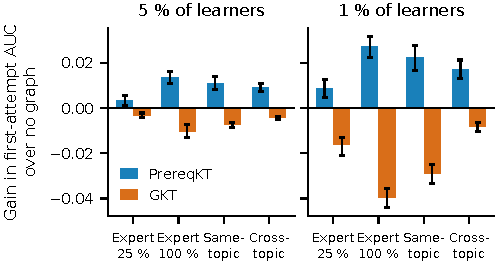
\includegraphics[width=\columnwidth]{fig4_architecture.pdf}
\caption{Gain in first-attempt AUC over no graph for the same graphs with PrereqKT and GKT (Junyi, 10 seeds, 95\% bootstrap intervals). Same-topic and cross-topic graphs are wrong graphs at 100\% coverage.}
\label{fig:arch}
\end{figure}

\begin{table}[t]
\centering
\caption{Coverage and Correctness Effects, Oriented in the Direction of the Graph's Effect (10 Seeds)}
\label{tab:magnitude}
\footnotesize
\setlength{\tabcolsep}{3.5pt}
\begin{tabular}{@{}llccccc@{}}
\toprule
Model & $\rho$ & Effect & Coverage & Correctness & Ratio & Seeds \\
\midrule
PrereqKT & 5\% & gain & 0.0103 & 0.0026 & 3.9 & 10/10 \\
PrereqKT & 1\% & gain & 0.0183 & 0.0047 & 3.9 & 9/10 \\
GKT & 5\% & loss & 0.0071 & 0.0027 & 2.6 & 10/10 \\
GKT & 1\% & loss & 0.0233 & 0.0106 & 2.2 & 9/10 \\
\bottomrule
\multicolumn{7}{@{}p{0.95\columnwidth}@{}}{\scriptsize Seeds: seeds in which the coverage effect exceeds the correctness effect ($p\le0.005$ in all rows).}
\end{tabular}
\end{table}

\subsection{Learned Graphs: Utility Without Recovery (RQ4)}
Edge weights learned end-to-end barely recover expert prerequisites, yet the learned graph is as useful for prediction as the expert graph (Fig.~\ref{fig:learned}, Tables~\ref{tab:recovery} and~\ref{tab:learnedkt}). With all learners, their ROC AUC is 0.538 and 0.536 with 5\% of learners: above chance in 5 of 5 seeds (H5 confirmed but weak, Holm $p<0.01$) and far below the practice-order statistic (0.803 and 0.714; H6 rejected, 0 of 5 seeds, two-sided $p<0.001$). Starting from the LLM scores and training on learner data degrades rather than improves fidelity (0.665 vs.\ 0.695 for the Qwen prior; H7 rejected, 0 of 5 seeds), and on pairs with variable order recovery is not distinguishable from chance after correction (H8: +0.021 and +0.022, Holm $p=0.29$ and $0.14$).

AUPRC and top-$K$ precision, which focus on the highest-ranked pairs that a graph would actually keep, confirm this picture (Table~\ref{tab:recovery}). The learned weights reach an AUPRC of 0.042 against a chance level of 0.036, and 4.7\% of their $K$ highest-ranked pairs are expert prerequisites. Practice order reaches about four times chance (0.142, 21.5\%), the Qwen score 0.080 and 12.2\%. Training from the LLM prior lowers top-$K$ precision from 12.2\% to 7.7\% with all learners and to 4.5\% with 5\% of learners. On pairs whose order varies, the learned weights remain at chance (AUPRC 0.055 vs.\ 0.050) while practice order keeps an advantage (0.172); on pairs with an imposed order, its advantage at the top of the ranking is small (0.225 vs.\ 0.219 for the Qwen score).

\textbf{Shape of the learned graphs.} Without prior, the weights are small and diffuse: the median weight is 0.02 (all learners) and 0.04 (5\%), the largest 0.62 and 0.34, and at most 0.01\% of pairs exceed 0.5. The NOTEARS term is close to zero ($h(W)=0.010$ and $0.105$), but the graph is not strictly acyclic: its $K=820$ highest-weighted pairs contain cycles through 34 and 70 items on average. With the LLM prior, training keeps many high weights inherited from the Qwen scores (3.8\% and 17.9\% above 0.5) and the penalty is far from satisfied ($h(W)=4.1$ and $1{,}525$), with hundreds of two-item cycles among pairs weighted above 0.1, although its top-$K$ pairs are acyclic. At $\lambda_{\mathrm{acyc}}=0.01$ the penalty therefore does not enforce acyclicity.

\begin{figure*}[t]
\centering
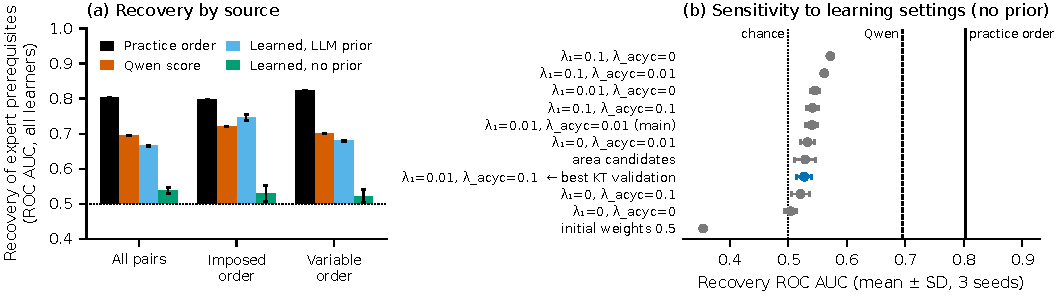
\includegraphics[width=\textwidth]{fig5_learned.pdf}
\caption{Recovery of expert prerequisites on Junyi. (a) ROC AUC by source and pair type, all learners, 5 seeds, 95\% bootstrap intervals; the dotted line is chance. (b) Learned graphs without prior under 11 learning settings (mean $\pm$ SD, 3 seeds); the highlighted setting has the best KT validation AUC, the pre-specified selection rule.}
\label{fig:learned}
\end{figure*}

\begin{table}[t]
\centering
\caption{Fidelity of Learned and Reference Scores on Junyi (All Learners, 5 Seeds)}
\label{tab:recovery}
\footnotesize
\setlength{\tabcolsep}{3.5pt}
\begin{tabular}{@{}lccc@{}}
\toprule
Source & ROC AUC & AUPRC & Top-$K$ precision \\
\midrule
Chance & 0.500 & 0.036 & 0.036 \\
Learned weights, no prior & 0.538 & 0.042 & 0.047 \\
Learned weights, LLM prior & 0.665 & 0.064 & 0.077 \\
Qwen score (the prior) & 0.695 & 0.080 & 0.122 \\
Practice order & 0.803 & 0.142 & 0.215 \\
\bottomrule
\end{tabular}
\end{table}

Weak recovery is not specific to one setting (Fig.~\ref{fig:learned}b). Across the nine combinations of $\lambda_1$ and $\lambda_{\mathrm{acyc}}$, recovery ranges from 0.50 to 0.57; the best setting ($\lambda_1=0.1$, $\lambda_{\mathrm{acyc}}=0$) reaches 0.572 with an AUPRC of 0.048. Initial weights of 0.5 give recovery below chance (0.355), and a larger candidate set (all pairs within a curriculum area, 184{,}524 pairs) gives 0.53. A strong acyclicity penalty brings $h(W)$ near zero without improving recovery. Meanwhile, KT performance hardly varies: validation AUC lies between 0.7945 and 0.7951 for all settings, so the selection rule cannot tell them apart, and the setting it picks recovers prerequisites with 0.527.

The learned graph is nonetheless as useful as the expert graph (Table~\ref{tab:learnedkt}). At $\rho=5\%$ it improves on no graph by 0.015 (5 of 5 seeds, $p=0.004$) and is at least as good as the expert graph (+0.003, 4 of 5 seeds, not significant); with all learners, no graph adds more than 0.002. Predictive gains from a learned graph are therefore not evidence that it encodes expert prerequisites. Nor is the high score of practice order evidence of prerequisite recovery: Junyi learners largely follow a curriculum built from the expert map, and the simulation (Section~\ref{sec:sim}) shows that this statistic tracks curriculum order rather than prerequisite effects.

\begin{table}[t]
\centering
\caption{First-Attempt AUC With Learned Graphs (PrereqKT, Junyi, 5 Seeds)}
\label{tab:learnedkt}
\footnotesize
\begin{tabular}{@{}lcc@{}}
\toprule
Graph & $\rho=5\%$ & $\rho=100\%$ \\
\midrule
No graph & 0.7650 & 0.8087 \\
Expert & 0.7773 & 0.8096 \\
Learned, no prior & 0.7799 & 0.8104 \\
Learned, LLM prior & 0.7797 & 0.8105 \\
\bottomrule
\end{tabular}
\end{table}

\subsection{Generalization to DBE-KT22}
On DBE-KT22, the reference relations are less useful than wrong relations of equal coverage, and all effects are small (Fig.~\ref{fig:dbe}). At full coverage, reference links underperform wrong cross-quiz links by 0.0011 ($\rho=20\%$, $p=0.03$) and 0.0049 (5\%, 0 of 10 seeds, $p<0.001$). Wrong links improve on no graph (+0.0018, +0.0028, Holm $p\le0.01$); reference links do not. Coverage helps modestly with wrong links only (partial $\eta^2=0.16$ at 20\%). With GKT ($\rho=20\%$), every graph again lowers AUC (reference $-0.0073$, wrong cross-quiz $-0.0254$); GKT could not be trained reliably with 44 students (5\%). Within its scope (undirected relatedness links), DBE-KT22 confirms that agreement with a reference graph does not make a graph more useful and that the direction of the effect depends on the architecture, but it does not reproduce the dominance of coverage, because effects are an order of magnitude smaller than on Junyi.

\begin{figure}[t]
\centering
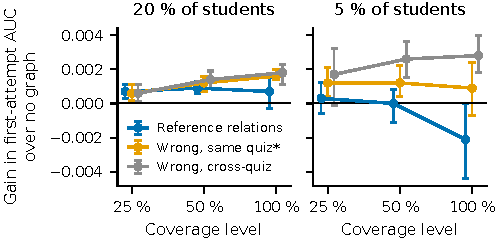
\includegraphics[width=\columnwidth]{fig6_dbe.pdf}
\caption{DBE-KT22 (PrereqKT, 10 seeds): gain in first-attempt AUC over no graph by coverage level. *Wrong same-quiz links are not matched in edge count, because quizzes are small.}
\label{fig:dbe}
\end{figure}

\subsection{Simulation: When Correctness Matters}
\label{sec:sim}
Correctness and direction matter only when prerequisites strongly affect success (Fig.~\ref{fig:sim}a, Table~\ref{tab:sim}). In S1, wrong same-topic edges keep 52\% of the ground-truth graph's benefit and reversed edges 61\%; in S2 and S3, correctness and direction have no detectable effect. On Junyi, wrong same-topic edges keep about 80\% of the benefit, a pattern closer to S2 and S3 than to S1. Recovery shows why log-based methods fail (Fig.~\ref{fig:sim}b). In S1 a simple statistic recovers the ground-truth prerequisites (practice-before: 0.86), yet the learned weights remain at chance (0.52) while yielding the same predictive gain as the ground-truth graph (+0.0084 vs.\ +0.0083): the prediction objective does not reward correct edges. Practice order recovers ``prerequisites'' only when the curriculum imposes them (0.72 in S3, where they have no effect; 0.51 in S1), co-occurrence lift falls below chance under strong prerequisites (0.29), consistent with the below-chance edge directions reported for co-occurrence statistics on Junyi~\cite{truong2026replication}, and even practice-before is inflated by an imposed order (0.63 in S3).

\begin{figure*}[t]
\centering
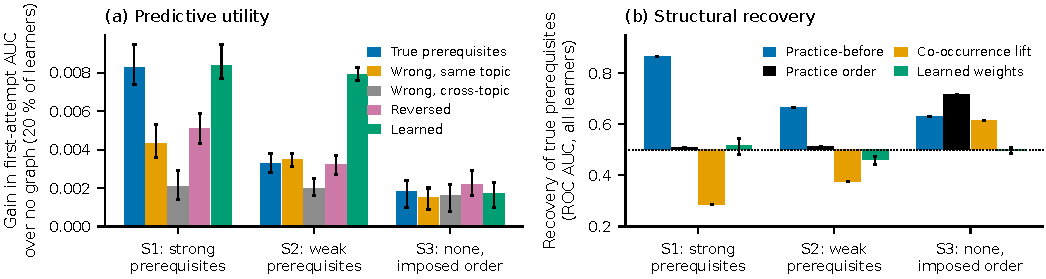
\includegraphics[width=\textwidth]{fig7_simulation.pdf}
\caption{Simulation (5 seeds, 95\% bootstrap intervals). (a) Gain in first-attempt AUC over no graph at 100\% coverage, PrereqKT, 20\% of learners. (b) Recovery of the ground-truth prerequisites (ROC AUC, all learners) by four methods.}
\label{fig:sim}
\end{figure*}

\begin{table}[t]
\centering
\caption{Effects on First-Attempt AUC in the Simulation (PrereqKT, $\rho=20\%$, 5 Seeds, Holm Correction Over 30 Tests)}
\label{tab:sim}
\footnotesize
\setlength{\tabcolsep}{3pt}
\begin{tabular}{@{}lccc@{}}
\toprule
Effect & S1 strong & S2 weak & S3 none \\
\midrule
Coverage (100\% $-$ 25\%) & +0.0064$^{*}$ & +0.0025$^{*}$ & +0.0016 \\
Correctness (expert $-$ same-topic) & +0.0040$^{*}$ & $-$0.0002 & +0.0003 \\
Proximity (same- $-$ cross-topic) & +0.0022$^{*}$ & +0.0014$^{*}$ & $-$0.0001 \\
Direction (expert $-$ reversed) & +0.0032$^{*}$ & +0.0001 & $-$0.0004 \\
\midrule
Benefit kept by same-topic edges & 52\% & 106\% & 83\% \\
\bottomrule
\multicolumn{4}{@{}l@{}}{\scriptsize $^{*}$Holm $p<0.05$, 5 of 5 seeds.}
\end{tabular}
\end{table}

\section{Discussion and Evaluation Guidelines}
\textbf{Why coverage dominates.} A first attempt on item $b$ can only be informed by other items. Any edge into $b$, correct or not, gives the model access to the learner's performance on related items, and same-topic items are informative about the learner's topical level whether or not they are formal prerequisites. Most of what a graph carries for prediction is thus evidence about general and topical ability; coverage determines how many first attempts receive it, and correctness only refines it. Learned graphs make the same point from the other direction: free to choose its edges, the model spreads small weights over the whole topic.

\textbf{Why the effect depends on the architecture.} PrereqKT treats the graph as an additional input that it can down-weight; GKT routes the learner's information through the graph. The same graph can therefore help one architecture and degrade another, at least in our implementation and regimes, while the relative importance of coverage and correctness is preserved. Claims that a graph is useful are claims about a graph and a model together.

\textbf{What the simulation says about real data.} When prerequisites strongly shape success, correct and correctly oriented edges are clearly better. On Junyi, the pattern resembles the weak- or no-prerequisite scenarios: the correctness data contain little exploitable prerequisite signal at the granularity of first attempts. The failure of learned graphs to recover prerequisites, however, is not explained by the data alone: in S1 the signal exists and a simple statistic finds it, but a diffuse graph achieves the same likelihood. Statistics computed on logs inherit the curriculum, so practice order can recover ``prerequisites'' that have no effect on success.

\textbf{Why small AUC differences matter here.} The absolute gains we compare are small (0.003--0.04 AUC), as is typical of graph effects in KT. Our contribution does not rest on their size but on their ordering: a structurally worse graph obtains the same or a larger gain than a better one, consistently across seeds. Such orderings are what published comparisons of graph-based KT rely on, so small differences are precisely where structure and utility can be confused.

\textbf{Implications for learning technologies.} LLM prerequisite judgements are better than chance, but their confident edges concentrate on a few foundational items, so the most precise graphs are the least useful for prediction; once coverage is equalized we detected no advantage of LLM-selected over random same-topic prerequisites (these comparisons were not equivalence tests). For KT, the value of an LLM or learned graph thus depends more on how its edges are distributed than on how accurate they are. For uses where correctness matters in itself, such as sequencing content, explaining a recommendation or planning remediation, graphs must be evaluated against expert references directly: a learned structure that improves prediction should not be presented to teachers or learners as pedagogical knowledge without structural evidence.

\textbf{Implications for interpretability claims.} Models that learn a prerequisite or concept graph jointly with prediction are often presented as interpretable. Our results caution against this reading when the only evidence is predictive performance: a learned graph matched the expert graph's benefit while recovering expert prerequisites barely above chance, under every setting we tried, both on Junyi and in a simulation where the ground-truth prerequisites were recoverable. This evidence concerns one family of learned-graph methods (sigmoid edge weights trained jointly with a KT model under sparsity and acyclicity penalties); it does not show that every graph learned by a KT model is pedagogically unfaithful, but it shows that predictive performance cannot establish faithfulness. Structural claims about learned graphs require structural evaluation.

\textbf{Evaluation guidelines.} We propose six practices for studies that use or produce prerequisite graphs for KT:
\begin{enumerate}
\item \emph{Evaluate where a graph can matter:} report first-attempt AUC and include sparse-data regimes; aggregate AUC with full data can hide graph effects.
\item \emph{Compare against coverage-matched random graphs:} same-topic and cross-topic, with the same number of edges per item.
\item \emph{Report a difficulty-only reference:} graph gains that do not exceed it mainly compensate for poor difficulty estimates.
\item \emph{Report coverage and concentration} of every graph, weighted by first attempts.
\item \emph{Evaluate structure directly} with ROC AUC, AUPRC and top-$K$ precision against expert annotations, and never infer it from predictive gains.
\item \emph{Include order-aware baselines} when recovering prerequisites from logs: practice order, and separate analyses of pairs with imposed and variable order.
\end{enumerate}

\section{Threats to Validity}
\label{sec:limits}
\textbf{External validity.} Junyi is the only public dataset we could identify with directed expert prerequisites, so the directed-prerequisite results rest on one platform and one domain, with a curriculum built from the same expert map. DBE-KT22 provides only symmetric relations, and the simulation relies on one generative model. \textbf{Construct validity.} Expert annotations can be incomplete; low fidelity indicates weak agreement with this reference, not that the relations are pedagogically wrong. LLM scores come from one prompt formulation and two mid-sized models. \textbf{Internal validity.} PrereqKT is our own instrument; we mitigated this with a published architecture (GKT), re-implemented with one reported adaptation. PrereqKT reads both prerequisites and successors, which lowers its sensitivity to direction. The sensitivity analysis of learned graphs used 3 seeds and all learners, did not cover the LLM-prior variant and did not try other optimization schemes such as the augmented Lagrangian of NOTEARS. S3 changes prerequisite strength and practice order at once. \textbf{Statistical conclusion validity.} Effects are small in absolute terms (0.003--0.04 AUC), so we used paired designs, Holm correction and seed counts; seeds resample training learners but not the test set, intervals over five seeds are coarse, and non-significant differences are reported as the absence of a detected advantage, not as equivalence. \textbf{Scope.} We study next-answer prediction; prerequisite graphs may matter more for sequencing, remediation or explanation.

\section{Conclusion}
We asked whether prerequisite graphs that agree more with experts are more useful for knowledge tracing, and whether graphs that help prediction reveal prerequisites. For the models, datasets and regimes we studied, neither relation held reliably. The utility of a graph for first-attempt prediction depended mainly on its coverage, which weighed two to four times more than correctness, and on how the architecture uses it. LLM graphs were more faithful than chance but showed no significant advantage over random same-topic graphs at equal coverage, and learned graphs, in the family of methods we studied, matched the expert graph's benefit while barely recovering expert prerequisites, under every learning setting we tried and in simulations where the ground-truth prerequisites were recoverable by a simple statistic. Structural quality and predictive utility should be treated as distinct properties and evaluated with distinct measures. Promising directions include datasets with richer expert annotations, uses of prerequisite graphs beyond prediction, and training objectives that reward structural correctness rather than predictive fit alone.

\section*{Acknowledgments}
The authors used Claude (Anthropic), a large language model, to assist with drafting and editing the text of this article and with writing analysis code. The authors reviewed, verified, and revised all content and take full responsibility for it.

\bibliographystyle{IEEEtran}
\bibliography{refs}

\end{document}
